\subsubsection{XML Import}
\par
The general idea with this utility is to import XML files into the a configured database. This will take any xml file or input stream convert them into java objects and then store them into an SQL database. The interface to this utility is an intiutive user interface where you can open, preview and import files. 
\begin{figure}[h]
	\centering
		\includegraphics[width=3.00in]{ImportUse.jpg}
	\caption{The Use Case For The Import Utility}
	\label{fig:Import Use}
\end{figure}



\par
The XML Import module is made up of two classes: the ImportPanel, and the ImportEngine. 

\begin{figure}[h]
	\centering
		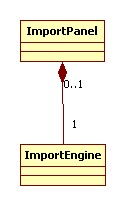
\includegraphics[width=1.00in]{ImportClasses.jpg}
	\caption{The ImportEngine is part of the ImportPanel but it can also run stand-alone}
	\label{fig:ImportClasses}
\end{figure}
